\documentclass[journal]{IEEEtran}

\usepackage[style=ieee]{biblatex} 
\usepackage{amsmath}
\usepackage{url}
\usepackage{graphicx}
\usepackage{float}

\usepackage[caption=false]{subfig}
\usepackage{todonotes}

% \bibliography{example_bib.bib}

\begin{document}

\title{Investigating Cross-Sectional Size Distribution of Randomly Distributed
       3D Spheres} 

\author{Sai Pandian, ID:\@ 29899923}%
        
% The report headers
\markboth{PHYS6017 Computer Techniques in Physics Report 2, May 2020}
% do not delete next lines
{Shell \MakeLowercase{\textit{et al.}}: Bare Demo of IEEEtran.cls for IEEE Journals}

\maketitle

\begin{abstract}
  Text
\end{abstract}

\section{Introduction}

\IEEEPARstart{I}{n} the world of Material Science and Crystallography, it is
often the case that a material is identified and classified using the
distribution of its constituent particle sizes. However, direct observation of
the particles so as to construct a distribution is often impossible. Using a
modern microscope or laser imaging techniques, it is possible to observe
particles in a cross-section of material. But the observed radii of particles in
this cross-section do not necessarily correspond directly to the radii of the
particles in the material, since the plane of the cross-section is not
necessarily oriented such that the observed particles lie exactly on the
plane. Thus, it becomes difficult to relate the observed distribution of
particle sizes in the plane to the real distribution of particle sizes in the
material.

Mathematically, determining the distribution of spherical particles from planar
sections is a well known problem called Wicksell's Corpuscle Problem
\todo{cite}, named after S. D. Wicksell, who solved the problem in 1925. With
this solution, it is possible to determine the original distribution of
spherical particles. Thus, it is possible to determmine the distribution of
particle sizes in a solid from its observed cross-section, allowing us to
identify and classify materials better \todo{nasa}.

In this paper we aim to show that it is possible to reproduce theoretical
results on cross-sectional distributions using numerical simulation, and it is
thus possible to solve Wicksell's Corpuscle Problem in this manner.


\section{Method}
Consider many spheres of different radii distributed randomly in space. For the
purposes of the numerical simulation, we will consider a cube of length 20. The
spheres were not allowed to overlap, which we ensured by placing the spheres such
that if one sphere has vector position $\overrightarrow{\textbf{a}}$ and radius
$r_{1}$ and the other has vector position $\overrightarrow{\textbf{b}}$ and
radius $r_{2}$, the spheres must have positions such that:
\begin{equation*}
|\overrightarrow{\textbf{a}} - \overrightarrow{\textbf{b}}| > (r_{1} + r_{2})
\end{equation*}
Random coordinates for a sphere are drawn from a uniform distribution and
checked against every existing sphere until a set of coordinates is drawn that
ensures no overlap, at which point the sphere is placed in space and the process
is repeated until all the necessary spheres have been placed.

\begin{figure}[H]%[!ht]
\begin{center}
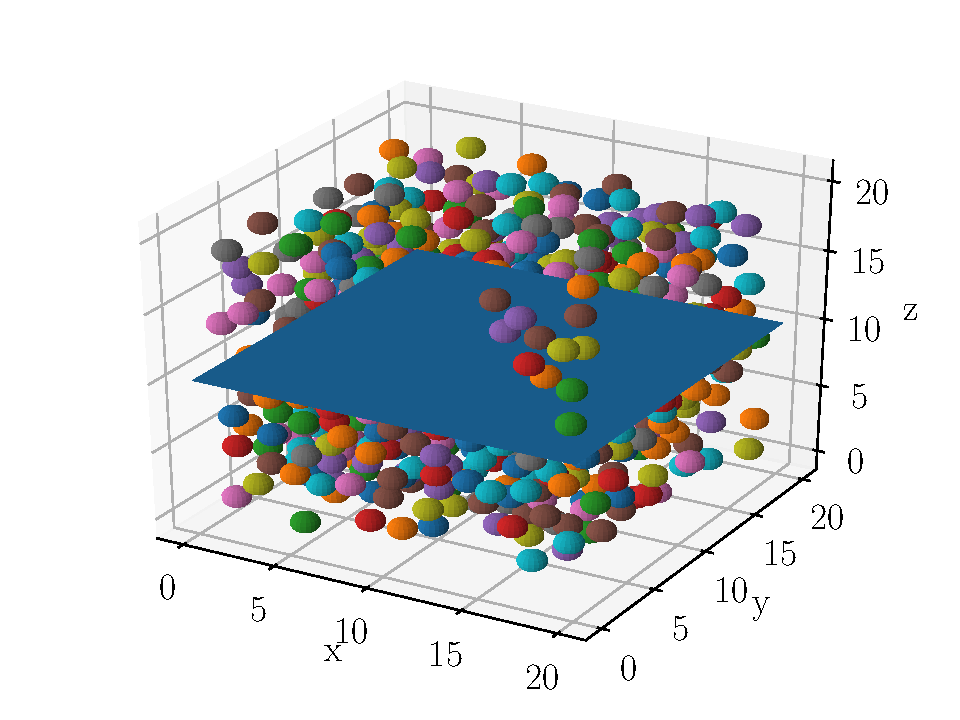
\includegraphics[width=0.45\textwidth]{./../Figures/box3d.pdf}
\caption{750 spheres of radius 0.7 distributed randomly in a cube of length 20,
  such that no sphere is touching or overlapping another sphere. A randomly
  oriented plane passes through the box and ``cuts'' through the
  spheres.}\label{fig:3dplot_plane}
\end{center}
\end{figure}

We then placed a plane into the cube, with a random orientation. The plane will
``cut'' through many of the spheres in the cube. This is shown in
Figure~\ref{fig:3dplot_plane}. Here we see 750 spheres, each with radius 0.7
distributed randomly in a cube of length 20. The plane is shown in blue, and can
be seen intersecting many of the spheres in the cube.

In order to obtain the planar cross-section, we employed the spherical cap
method \todo{cite}. If we consider a sphere with centre
$\overrightarrow{\textbf{c}_0} = (x_0, y_0, z_0)$ and radius $R$, and a plane
with equation $Ax + By + Cz = D$ such that $\overrightarrow{\textbf{n}} = (A, B,
C)$ is the normal vector to the plane, then the distance from the centre of the
circle to the closest point on the plane $p_0$ is given by $\rho$:
\begin{equation*}
\rho = \frac{(\overrightarrow{\textbf{c}_0} - \overrightarrow{\textbf{p}_0}) \cdot{}
  \overrightarrow{\textbf{n}}}{|\overrightarrow{\textbf{n}}|} = \frac{Ax_0 +
  By_0 + Cz_0 - D}{\sqrt{A^2 + B^2 + C^2}}
\end{equation*}
If $|\rho| < R$, then there is an intersection of the plane and the sphere. The
radius of the circle $r$ in the planar cross-section is given by:
\begin{equation*}
r = \sqrt{R^2 - \rho^2}
\end{equation*}
And we then binned this radius to produce a histogram of the distribution of
planar circle radii. It is also possible to recover the centre
$\overrightarrow{\textbf{c}}$ of the circle visible on the plane using:
\begin{equation*}
\overrightarrow{\textbf{c}} = \overrightarrow{\textbf{c}_0} +
\rho\frac{\overrightarrow{\textbf{n}}}{|\overrightarrow{\textbf{c}}|} = (x_0,
y_0, z_0) + \rho\frac{(A, B, C)}{\sqrt{A^2 + B^2 + C^2}}
\end{equation*}

\begin{figure}[H]%[!ht]
\begin{center}
\includegraphics[width=0.45\textwidth]{./../Figures/circles.pdf}
\caption{Planar cross-section constructed using mock data. Spheres cut by the
  plane appear as circles on the plane, with radius dependent on the relative
  position of the spheres to the plane. This distribution of circles can be
  modelled.}\label{fig:circles}
\end{center}
\end{figure}

Figure~\ref{fig:circles} presents a planar cross-section generated using this
method and mock data. As we see, there are a range of circular radii observed
since even though the spheres all had the same radius, they were at different
distances from the plane, and were thus cut at different points. The many
observed circular radii are binned to produce a distribution.

If $f(R)dR$ is the number of spheres per unit volume with radii in interval $[R,
R + dR]$, then we can define a distribution $\phi(x)dx$ which represents the
number of circles per unit area on the plane with radii in interval $[x,
x+dx]$ \todo{cite}. This distribution is given by:
\begin{equation}
\phi(x) = \int_{x}^{\infty}\frac{xf(R)}{\sqrt{R^2 - x^2}}
\label{eq:phi_OG}
\end{equation}
We can compute this integral to obtain a theoretical planar distribution for
different starting spherical radius distributions.

We first considered the case in which all the spheres had the same radius
$R_0$. In this case, the spherical radius distribution is simply a Dirac delta
function centred on the radius $R_0$.

If we compute the integral in Equation~\ref{eq:phi_OG}, replacing $f(R)$ with
$\delta(R-R_0)$ we find:
\begin{equation}
\phi(x) = \int_{x}^{\infty}\frac{x\delta(R-R_0)}{\sqrt{R^2 - x^2}} =
\frac{xH(R_0-x)}{\sqrt{R_0^2-x^2}}
\label{eq:phi_constant}
\end{equation}
where $H(R_0 - x)$ is the heaviside function, which ``turns on'' the
distribution only for $x < R0$ as it is not possible to have a circular radius
$x$ larger than the spherical radius. So we aim to see our experimental data
reproduce this distribution \todo{cite}. We also investigated how changing the
value of $R_0$ affects the experimental distribution.

We next considered the case in which each sphere has a radius $R$ uniformly
distributed in a range $R_1 < R < R_2$. In this case, we modify $f(R)$ in
Equation~\ref{eq:phi_OG} to be:
\begin{equation*}
  f(R) =
  \begin{cases}
    1,& \text{if } R_1 < R < R_2\\
    0,& \text{} Otherwise
  \end{cases}
\end{equation*}
In this case the integral in Equation~\ref{eq:phi_OG} does not need to be
computed with the limits shown, but instead with limits between $R_1$ and $R_2$
since $f(R)$ is 0 otherwise:

\begin{equation}
\begin{split}
  \phi(x) & = \int_{R_1}^{R_2}\frac{xf(R)}{\sqrt{R^2 - x^2}} \\
  = x\ln\left(\sqrt{R_2^2 - x^2}+R_2\right) & - x\ln\left(\sqrt{R_1^2 - x^2}+R_1\right)
\end{split}
\end{equation}
Since this distribution produces complex numbers for $ x < R_1$, we only
consider the real part of this distribution, which appears to produce a peak at
$x = R_1$.

\section{Results}
Text

% \begin{figure}[H]%[!ht]
% \begin{center}
% 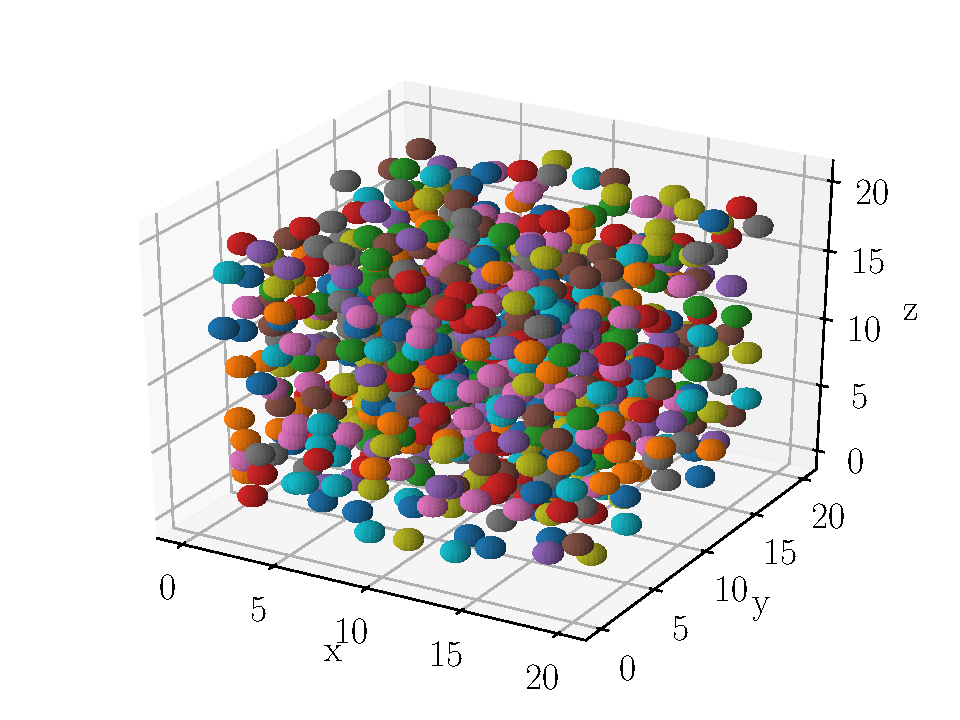
\includegraphics[width=0.45\textwidth]{./../Figures/box3d_noplane.pdf}
% \caption{Spheres of radius 0.7 distributed randomly in a cube of length 20, such
%   that no sphere is touching or overlapping another sphere.}
% \label{fig:3dplot}
% \end{center}
% \end{figure}

\begin{figure}[H]%[!ht]
\begin{center}
\includegraphics[width=0.45\textwidth]{./../Figures/750_01.pdf}
\caption{Distribution of circle radii on plane for 750 spheres of radius $0.1$
  each. There are relatively few points since the spheres are small, so there is
  relatively small chance that they will be cut by the plane. So only a few
  circles are visible on the plane. The theoretical distribution is shown, with
  the experimental data matching this distribution, showing a slow increase in
  number or circles as radius increases.}\label{fig:size1}
\end{center}
\end{figure}

\begin{figure}[H]%[!ht]
\begin{center}
\includegraphics[width=0.45\textwidth]{./../Figures/750_03.pdf}
\caption{Distribution of circle radii on plane for 750 spheres of radius $0.3$
  each. Compared to Figure~\ref{fig:size1}, there are many more experimental data
  points, since it is more likely that the plane will intersect these larger
  spheres. The experimental data more clearly resembles the theoretical
  distribution, showing a strong increase in number of circles as radius
  increases towards the maximum of 0.3.}\label{fig:size3}
\end{center}
\end{figure}

\begin{figure}[H]%[!ht]
\begin{center}
\includegraphics[width=0.45\textwidth]{./../Figures/750_07.pdf}
\caption{Distribution of circle radii on plane for 750 spheres of radius $0.7$
  each. We do not observe much difference in how well the experimental data
  resembles the theoretical distribution between this figure and
  Figure~\ref{fig:size3}. With larger sized spheres, the simulation becomes harder
  to run as it is more difficult to randomly place spheres in a finite space
  without overlap.}\label{fig:size7}
\end{center}
\end{figure}

\begin{figure}[H]%[!ht]
\begin{center}
\includegraphics[width=0.45\textwidth]{./../Figures/750_07_random.pdf}
\caption{Distribution of circle radii on plane for 750 spheres of radius $R$
  where $0.65 < R < 0.7$. The theoretical distribution is now different,
  although the experimental data still resembles this new distribution, showing
  a maximum around $R = 0.7$ and a sharp decrease after this. This is likely
  because there are more spheres with radii such that an overlap between $0$ and
  $0.7$ is possible, and relatively few spheres with radii such that a larger
  overlap is possible.}
\label{fig:random}
\end{center}
\end{figure}

% \begin{figure}[H]%[!ht]
% \begin{center}
% \includegraphics[width=0.45\textwidth]{./../Figures/750_07_NoNoise.pdf}
% \caption{Illustrations, graphs, and photographs may fit across both columns, if
%   necessary. Your artwork must be in place in the article.}
% \label{fig:nonoise}
% \end{center}
% \end{figure}

% \begin{figure}[H]%[!ht]
% \begin{center}
% \includegraphics[width=0.45\textwidth]{./../Figures/750_07_Noise_100.pdf}
% \caption{Illustrations, graphs, and photographs may fit across both columns, if
%   necessary. Your artwork must be in place in the article.}
% \label{fig:2noise}
% \end{center}
% \end{figure}

% \begin{figure}[H]%[!ht]
% \begin{center}
% \includegraphics[width=0.45\textwidth]{./../Figures/750_07_Noise_10.pdf}
% \caption{Illustrations, graphs, and photographs may fit across both columns, if
%   necessary. Your artwork must be in place in the article.}
% \label{fig:1noise}
% \end{center}
% \end{figure}

\begin{figure*}[ht!]
  \centering
  \subfloat[Noise 2 orders of magnitude smaller than radius]
  {\includegraphics[width=0.45\textwidth]{./../Figures/750_07_Noise_100.pdf}
  \label{fig:2noise}}
  \centering
  \subfloat[Noise 1 order of magnitude smaller than radius]
  {\includegraphics[width=0.45\textwidth]{./../Figures/750_07_Noise_10.pdf}
  \label{fig:1noise}}
  \caption{Distribution of circle radii on plane for 750 balls of radius $0.7$
    each. Each recorded radius has a random noise added to it in order to
    determine how sensitive the data is to experimental
    error. Figure~\ref{fig:2noise} shows the distribution for an added noise 2
    orders of magnitude smaller than the recorded radius, while
    Figure~\ref{fig:1noise} is the same for noise 1 order of magnitude smaller. As
    we can see, the experimental data very resembles the theoretical
    distribution when noise of 2 orders of magnitude smaller are added. But this
    is not true when noise of 1 order of magnitude smaller is added, implying
    the data is very sensitive to experimental data.}
  \label{fig:noiseplots}
\end{figure*}

\section{Discussion and Summary}
Text



% if have a single appendix:
%\appendix[Proof of the Zonklar Equations]
% or
%\appendix  % for no appendix heading
% do not use \section anymore after \appendix, only \section*
% is possibly needed

% use appendices with more than one appendix
% then use \section to start each appendix
% you must declare a \section before using any
% \subsection or using \label (\appendices by itself
% starts a section numbered zero.)
%
\appendices{}
\section{Appendix Name}
Text

\printbibliography{}
\end{document}
